%%%%%%%%%%%%%%%%%%%%%%%%%%%%%%%%%%%%%%%%%%%%%%%
% These are the general sections to include.  %
%                                             %
% You can alter some names, but follow the    %
% suggestions in the NSF guidelines.          %
%                                             %
% If spacing is tight, play with negative     %
% vspaces w/in the text to reduce whitespace. %
%%%%%%%%%%%%%%%%%%%%%%%%%%%%%%%%%%%%%%%%%%%%%%%

%%%%%%%%%%%%%%%%%%%%%%%%%%%%%%
% Section 1: Introduction    %
%%%%%%%%%%%%%%%%%%%%%%%%%%%%%%
\section{Introduction}
\label{intro}



%%%%%%%%%%%%%%%%%%%%%%%%%%%%%%
% Section 2: Overview        %
%%%%%%%%%%%%%%%%%%%%%%%%%%%%%%
\section{Background}

\subsection{GPU design principles}
There are four major design principles to consider when implementing data
structures on GPUs:

\begin{enumerate}[noitemsep, leftmargin=*]
    \item \textbf{Low thread divergence:} threads inside a warp should execute
      the same instruction. This enables writing simple kernels that can exploit
      massive parallelism in the GPU\@.
    \item \textbf{High memory coherence:} threads inside a warp should access
      the same  memory from a local region. Random memory accesses are expensive
      and cause threads to stall.
    \item \textbf{High degree of parallelism:} a high number of threads saturate
      memory bandwidth and hide memory latency.
    \item \textbf{Atomic operations:} atomic operations help efficient thread
      scheduling inside a warp. Non-atomic writes and data movements cause slow
      downs and require locking large memory regions. Locking results in high
      overheads and affects the overall throughput.
    \end{enumerate}

\john{Contention! Avoiding contention given the number of concurrent threads is huge.}

\subsection{A Brief History of Filters}\label{sec:prelim}

Filter data structures can be broadly classified into \emph{static} and
\emph{dynamic}.  Static filters approximately represent a set of items that must
be known before building the filter. Examples of these filters include XOR
filters~\cite{GrafLe20} and Ribbon filters~\cite{DillingerWalzer21}. Static
filters have recently seen more advancement due their use in storage
applications, such as LSM-trees.


In this paper, we consider dynamic filters as they have wide-spread applications
in data analytics.  Dynamic filters approximately represent a set of items that
does not need to be known before the construction. Dynamic filters have seen
much more advancement in the last few decades as applications often do not know
the set of items in advance. Examples of dynamic filters are Bloom
filters~\cite{Bloom70}, quotient filters~\cite{BenderFaJo12,
PandeyBJP17b,DillingerMa09,PaghPaRa05,EinzigerFr16}, and cuckoo
filters~\cite{FanAnKa14,BreslowJ18}.

\textbf{Bloom filters} consume $\log(e)\, \opt$ space, which is roughly
$\log(e)\approx 1.44$ times more than the lower bound of $\opt + \Omega(n)$
bits~\cite{CarterFG78}. In contrast, for a set $S$ taken from a universe $U$,
where $|U|=u$, an error-free dictionary requires $\Omega(\log {u\choose n})
\approx \Omega(n \log u)$ bits. Bloom filters also incur $\errbits$ cache-line
misses on inserts and positive queries, giving them poor insertion and query
performance.

\textbf{Blocked Bloom filters}~\cite{putze2007cache} overcome the poor cache
locality of Bloom filters by constructing a series of smaller Bloom filters each
of which is small enough to fit inside a small number of cache lines. The first
hash function is used to select a block and rest of the hash functions are used
to set/test bits inside the block. However, the cache efficiency comes at the
cost of higher false-positive rate. Blocked Bloom filters have theoretically and
empirically higher (up to $5\times$) false positive rates compared to Bloom
filters. See \Cref{tab:merged_fp_space} for the empirical calculations of FP
rate.

\textbf{Quotient
filters}~\cite{Cleary84,PaghPaRa05,DillingerMa09,BenderFaJo12a,PandeyBJP17,pandeySigmod21}
represent a set approximately by compactly storing small fingerprints of the
items in the set via Robin Hood hashing~\cite{CelisLaMu85}. The quotient filter
uses $1.053 (2.125 + \log_21/\epsilon)$ bits per element, which is less than the
Bloom filter whenever $\epsilon \leq 1/64$, which is the case in almost all
applications. It supports insertion, deletion, lookups, resizing, and merging.
The counting quotient filter (CQF)~\cite{PandeyBJP17}, improves upon the
performance of the quotient filter and adds variable-sized counters to count
items using asymptotically optimal space, even in large and skewed datasets. In
the counting quotient filter, we can also associate small values with items
either by re-purposing the variable-sized counters~\cite{PandeyABFJP18Cell} to
store values or by explicitly storing small values with the remainders in the
table~\cite{PandeySMB20}.

\textbf{Cuckoo filters}~\cite{FanAnKa14,BreslowJ18} also store small
fingerprints compactly in a table. However, unlike the quotient filter that uses
Robin Hood hashing, the cuckoo filter uses cuckoo hashing to resolve collisions
among fingerprints. Cuckoo hashing uses kicking (or cuckooing) to find an empty
slot for the new item when all the slots in a bucket are occupied. This results
in a cascading sequence of kicks until the filter converges on a new stable
state. Inserts become slower as the structure becomes full, and in fact inserts
may fail if the number of kicks during a single insert exceeds a specified
threshold (500 in the author's reference implementation).

\textbf{Two-Choice filters}~\cite{pandeySigmod21} organize fingerprints
compactly in blocks similar to the cuckoo filter. However, unlike the cuckoo
filter, there is no kicking. The blocks in the two-choice filter are larger in
size ($\approx \log{n}$, where $n$ is the number of items which is usually the
size of the cache line on most machines) than the cuckoo filter and
power-of-two-choice hashing is used to reduce the variance across the blocks and
achieve a high load factor. During insertions if both blocks corresponding to a
fingerprint are full then the data structure is declared full. The
power-of-two-choice hashing enables the filter to probe exactly two cache lines
during inserts and queries and write to a single cache line during inserts.
Given the larger block sizes the vector quotient filter~\cite{pandeySigmod21}
uses quotienting (similar to the quotient filter) to organize fingerprints
inside blocks. It divides the fingerprints into a quotient and remainder part
and only stores the remainder in the slot given by the quotient. It uses two
additional metadata bits to resolve collisions among quotients.


\subsection{Analysis of filter designs}

We now look at the dynamic filters discussed in~\Cref{sec:prelim} and evaluate
them based on the GPU design principles.  Our goal is to identify the filters
that offer necessary features such as deletions, counting, and value
associations and at the same time satisfy most of the design principles.  We
will further discuss the challenges of implementing these filter on the GPUs to
achieve high speed operations.

Bloom filters are easy to implement on the GPU as they only require test and set
operations. These operations can be implemented using atomic operations and
achieve low thread divergence. However, each operation results in multiple cache
misses and therefore Bloom filters have low memory coherence. They also have
sub-optimal space usage. Moreover, Bloom filters do not support deletions,
counting\footnote{The counting Bloom filter~\cite{FanCaAl00}, a variant of the
Bloom filter, supports counting but it comes at a high space-overhead which
makes it highly inefficient in practice.}, and associating small values with
items.
% that many data analytics applications require.

Blocked Bloom filters are better suited to GPUs.  Each operation requires
probing inside a single block. They achieve low thread divergence, high memory
coherence, a high degree of parallelism, and atomic operations. Thus, blocked
Bloom filters can satisfy all the GPU design principles. However, blocked Bloom
filters have a high false-positive rate compared to Bloom filters and also do
not support necessary features like deletions and counting.

Operations in the quotient filter have high cache locality which makes it an
appropriate choice to achieve high memory coherence. However, insert operations
in the quotient filter requires shifting fingerprints which makes it harder to
use atomic operations and also results in high thread divergence. However, the
quotient filter can support all the necessary features like deletions, counting,
and associating small values with items which makes the quotient filter a highly
usable data structure that multiple applications can benefit from.

It is quite challenging to achieve high speed operations while maintaining all
of the features in a GPU implementation of the quotient filter. Geil et
al~\cite{Geil:2018:QFA} implemented a preliminary version of the GPU quotient filter.
However, that implementation was adapted from Bender et al.'s quotient
filter~\cite{BenderFaJo12a}, which did not have all the features, like counting
and value association, and also had higher space overhead. Furthermore, Geil et
al.'s GPU-based quotient filter has implementation-specific limitations (e.g., it
supports a fixed false-positive rate and can only be sized to store less than
$2^{26}$ items) resulting in poor performance and limited scalability.

The cuckoo filter stores fingerprints in fixed size blocks. This design is
amenable to high memory coherence and low thread divergence. Atomic operations
can also be used to read and write fingerprints. However, the cascading sequence
of reads and writes to random memory locations makes the cuckoo filter hard to
implement efficiently on the GPU\@. In particular, at high load factors when the
number of kicked items becomes high, each insertion will result in very low
memory coherence. Moreover, each kicking operation results in multiple
cache-line writes. This makes it challenging to achieve high speed operations in
a GPU cuckoo filter. Moreover, cuckoo filters do not support counting and
associating small values with items.

The two-choice filter has the advantages of the cuckoo filter design. It has
fixed size blocks. Each operation requires probing into exactly two blocks, and
inserts and deletes only write into a single block. This results in low thread
divergence, high memory coherence, and a high degree of parallelism. However,
due to large block sizes a more sophisticated structure is required to maintain
fingerprints inside each block. Therefore, it is not straightforward to use
atomic operations to read or write fingerprints inside blocks. It is a
challenging task to implement a two choice filter on the GPU using atomic
operations to achieve high throughput.




\section{Applications}

\subsection{MetaHipMer}

Metagenome assembly involves reconstructing long contiguous sequences ({\it
contigs}) of genetic material from short input {\it reads}. These reads are
strings of bases (the DNA alphabet A,C,G,T) of length 150 to 250 that are
produced by gene sequencing machines.  For metagenomes, these reads are
extracted from environmental samples (e.g. gut bacteria, or a soil sample) that
contain the genes of potentially thousands of microbes, existing at varying
abundances.  The reads are error prone (typically about 0.24\% error per base)
and sequencing is done multiple times to ensure every region of genetic material
is covered with some error free sequences.

In the approach used by MetaHipMer, the reads are first divided into overlapping
substrings of fixed length {\it k}, called {\it $k$-mers}, which are then used
to form a de Bruijn graph~\cite{CompeauPeTe11}. In a de Bruijn graph, the
vertices are $k$-mers and edges connect any two $k$-mers that have an overlap of
$k-1$ bases. These vertices are stored in a hash table that is distributed
across all the compute processes.  The size of the hash table is dependent on
the number of unique $k$-mers.  Traversal of the de Bruijn graph enables the
construction of the contigs (longer sequences).  This approach is more efficient
than an all-to-all alignment of the reads, which would be prohibitive for the
size of typical metagenome datasets (up to billions of reads).

Forward and backward extensions of the $k$-mer and the counts of those
extensions are also maintained in the hash table along with the $k$-mer.
Information regarding the extensions and their counts is critical to identifying
correct paths in the de Bruijn graph and requires 28 to 52 bytes (depending on
$k$) to store each $k$-mer.

To ensure accurate contigs, the $k$-mers that occur only once (singletons) are
treated as errors and dropped. In a typical set of metagenome reads, 70 to 80\%
of unique $k$-mers are singletons, but they still need to be stored and counted
in the distributed hash table. In the default MetaHipMer implementation, storing
the unique $k$-mers is the most memory intensive part of the computation and can
be roughly an order of magnitude larger than the input data.  The space required
to store the $k$-mers can be much larger than the size of the original raw
dataset (up to $10\times$ larger) as $k$-mers contain a lot of redundant
information due to their overlaps.

The distributed hash table in MetaHipMer is implemented as a collection of local
hash tables, one per process, with communication happening via UPC++ remote
procedure calls (RPCs). In the hash table insertion phase, the $k$-mers are
aggregated, dispatched over the network, and inserted in bulk into the local
hash tables, which are running on GPUs. Using GPUs boosts performance, but
further constrains memory (e.g. the Summit supercomputer~\cite{VazhkudaiDBG18}
has an aggregate of 96GB GPU memory and 512GB CPU memory per node).

MetaHipMer runs on distributed systems with multiple nodes, and each node could
have multiple GPUs, e.g. Summit has 6 GPUs per node. To utilize all the GPUs on
a node, MetaHipMer maps the UPC++ processes to the GPUs in a round robin
fashion, so multiple processes will share each GPU using the Nvidia
Multi-Process Service (MPS). On a Summit node there will be 42 processes (one
per core) and hence there will be 7 processes per GPU\@. Using the MPS has the
benefits of simplicity, because there is no inter-GPU communication required,
and it improves performance by increasing the utilization of the GPUs.

\Cref{fig:mhm-kmer} shows different parts of the $k$-mer analysis phase in
MetaHipMer. In the standard pipeline, all $k$-mers are counted in the hash table
and then a separate phase is required to purge all the singleton $k$-mers.

\subsection{$k$-mer distribution}

\Cref{tab:kmer-dist} shows the distribution of singleton $k$-mers in three
different metagenomic datasets. Singleton $k$-mers form a majority fraction of
the total number of distinct $k$-mers. The distribution often depends on the
sequencing depth and the size of $k$. The larger value $k$ results in larger
fraction of singleton $k$-mers. This is due to the higher probability of seeing
an erroneous base in the $k$-mer given the higher value of $k$. The erroneous
bases result in singleton $k$-mers.

Weeding out singleton $k$-mers before inserting them in the hash table to count
is critical in any $k$-mer analysis phase to reduce the memory usage of the
counting phase. These singleton $k$-mers can also be pruned from the hash table
after the counting phase. However, that results in the high peak memory usage
and much slower running time.

Using a space-efficient filter to weed out singleton $k$-mers helps to reduce
the memory pressure on the counting hash table thereby reducing the peak memory
usage and increased run time. See~\cref{fig:mhm-kmer}.


%%%%%%%%%%%%%%%%%%%%%%%%%%%%%%
% Section 3: Research Plan   %
%%%%%%%%%%%%%%%%%%%%%%%%%%%%%%
\section{Research Methodology}


\subsection{A component of your plan}


\setlength\intextsep{0pt}
\begin{wrapfigure}[20]{R}{2.4in}
\vspace{-5pt}
\centering
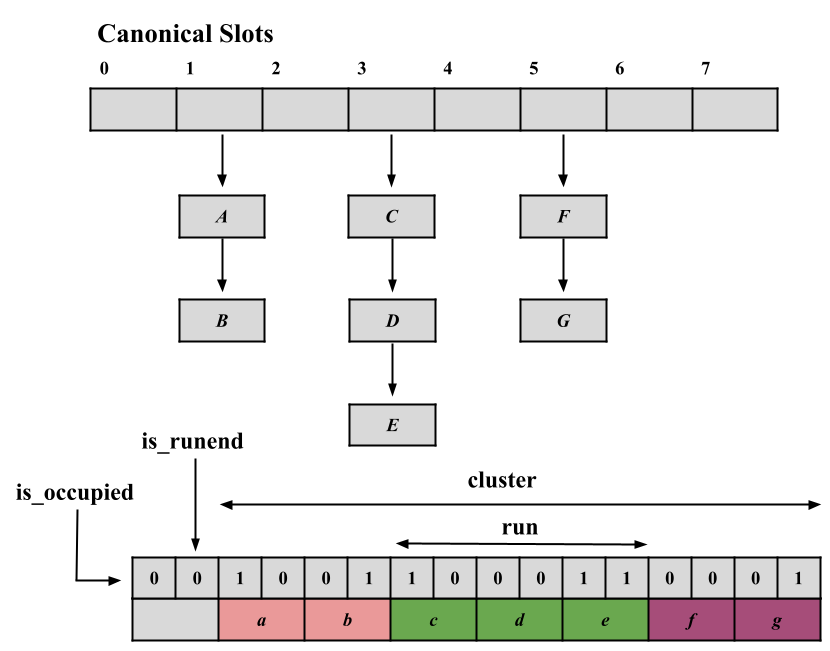
\includegraphics[width=2.4in]{images/canonical_slots}
\caption{Quotient filter block diagram.}
\label{fig1}
\end{wrapfigure}




\begin{wraptable}[15]{r}[0.01in]{4.5in}
\label{table1}
\caption{A sample table wrapped by text.}
\begin{center}
\vspace{-10pt}
\scriptsize
\begin{tabular}{  c  c  c  }
\hline
\hline
Stability & $M_u$ & $M_{\tau}$ \\
\hline\hline\\
Neutral & $\cfrac{z}{z_\Delta} - \cfrac{\ln(z/z_o)}{\ln(z_\Delta/z_o)}$ & $\cfrac{z}{z_\Delta} - \cfrac{1}{\ln(z_\Delta/z_o)}$\\\\
\hline \\
Stable & $\left(1 - \cfrac{\Psi}{2}\right)\cfrac{z}{z_\Delta} - \left(1 - \cfrac{\Psi_\Delta}{2}\right)
\left(\cfrac{\ln(z/z_o)-\Psi}{\ln(z_\Delta/z_o)- \Psi_\Delta}\right)$ & $\cfrac{z}{z_\Delta} - \cfrac{\left(1 - \cfrac{\Psi_\Delta}{2}\right)}{\ln(z_\Delta/z_o) - \Psi_\Delta}$\\\\
\hline \\
Unstable & $\cfrac{4}{3}\left[\left(\cfrac{1-x^3}{1-x_{\Delta}^{4}}\right) -  \left(\cfrac{1-x_{\Delta}^3}{1 - x_{\Delta}^{4}}\right)\left(\cfrac{\ln(z/z_o)-\Psi}{\ln(z_\Delta/z_o)- \Psi_\Delta}\right)\right]$ & $\cfrac{z}{z_\Delta} - \cfrac{\cfrac{4}{3}\left(\cfrac{1-x_{\Delta}^3}{1 - x_{\Delta}^{4}}\right)}{\ln(z_\Delta/z_o) - \Psi_\Delta}$\\\\
\hline
\hline
\end{tabular}
\end{center}
\end{wraptable}



% I found it useful to include a summary of the proposed work
% given in each subsection to help out reviewers.
\subsubsection{Specific tasks for this research component}
\begin{itemize}
\setlength\itemsep{0em}
\item Do a thing and blow your mind
\item Question your life choices
\item Drink coffee
\end{itemize}

\begin{center}
\begin{minipage}{.3\textwidth}
\begin{equation}
 \bar u = \bar u_{ll} + u_* \beta M_{u} \label{new_u}
\end{equation}
\end{minipage}
\begin{minipage}{.36\linewidth}
\begin{equation}
  \tau_{xz} = u_* u_{*ll} + \kappa u_*^2 \beta M_{\tau} \label{new_tau} \mbox{ ,}
\end{equation}
\end{minipage}
~\\Sample equations that consume minimal space.
\end{center}



%%%%%%%%%%%%%%%%%%%%%%%%%%%%%%
% Section 4: Management Plan %
%%%%%%%%%%%%%%%%%%%%%%%%%%%%%%
\section{Time Line and Management Plan}

\begin{table}[H]
\label{table1}
\renewcommand{\arraystretch}{0}
\caption{Project schedule.  PIs are Person One (P1), Person Two (P2), graduate student is GS, and the undergraduate student is US\@. Time frame gives the year each activity will occur.}
\scriptsize
\begin{tabularx}{\textwidth}{Y c c }
\hline
\hline
\textbf{Research Activity} & \textbf{Personnel} & \textbf{Time Frame}\\
\hline
Perform a task that sounds impressive & P2, US & Y1 \T\\
Perform another super-amazing task & P1, US & Y1 \T\\
Perform something else that may not be as sexy as the other things & P2, GS & Y1 \T\\
Wonder why you are such a terrible programmer & P1, US & Y1 \T\\
Analyze the results and stuff & P1, P2, SS & Y1,Y2 \T\\
Take the day off and grill some meat & P1, P2, SS & Y1,Y2 \T\\
Present findings at scientific meetings and publish results in peer-reviewed journals & P1, P2, US, GS & Y1, Y2, Y3\T\B\\
\hline
\hline
\end{tabularx}
\end{table}

%%%%%%%%%%%%%%%%%%%%%%%%%%%%%%
% Section 5: Science Merit   %
%%%%%%%%%%%%%%%%%%%%%%%%%%%%%%
\section{Scientific Merit}


%%%%%%%%%%%%%%%%%%%%%%%%%%%%%%
% Section 6: Impact/Outreach %
%%%%%%%%%%%%%%%%%%%%%%%%%%%%%%

\section{Broader Impacts}
\label{broadimpacts}
\vspace*{-8pt}

This project will have direct impacts on research and education through access to simulation data products, student training, and K-12 outreach.

\vspace{4pt}
\noindent \underline{\textit{Data Access}}: Maybe write about you will make data available.

\vspace{4pt}
\noindent \underline{\textit{Student Training}}: Write about how you will train students.

\vspace{4pt}
\noindent \underline{\textit{Some Other Outreach}}: Write about more outreach.

\vspace{4pt}
\noindent \underline{\textit{Dissemination}}: Write about how you will disseminate results (i.e., journal articles, workshops, etc).

%%%%%%%%%%%%%%%%%%%%%%%%%%%%%%
% Section 7: Prior NSF Work  %
%%%%%%%%%%%%%%%%%%%%%%%%%%%%%%
\section{Results from Prior NSF Support}

\noindent \emph{\underline{Person One}}: No NSF support in the past five years \newline

\noindent The most relevant prior NSF award to the proposed project for
\underline{Person Two} (Co-PI) is: (a) NSF PDM \#\#\#\#\#\#\#, \$000,000,
MM/DD/YY to MM/DD/YY; (b) Title: Super Cool Project That Got Funded; (c)
Accomplishments related to the {\bf intellectual merit} of this research project
include something something. The {\bf broader impacts} include outreach at many
levels. Something Something. To date, the grant has funded one post-doc and 1000
graduate students. The project has also involved 500 undergraduate students. (d)
To date this project has resulted in 100 conference presentations, one million
journal publications (cite them) with one under review (cite it) and two in
preparation with well-developed drafts.

% \nocite*
% don't do that
